\documentclass[12pt]{article}

% Computational Physics by M. Newman
% Setup file for exercises

% Packages
\usepackage{mathpazo}
\usepackage{amsmath}
\usepackage{graphicx}
\usepackage{calrsfs}
\usepackage{fancyvrb}

% Formatting
\setlength{\textwidth}{17.5cm}
\setlength{\textheight}{24.0cm}
\setlength{\evensidemargin}{2.5cm}
\setlength{\oddsidemargin}{-0.6cm}
\setlength{\topmargin}{-2.3cm}
\setlength{\textfloatsep}{0pt}
\setcounter{secnumdepth}{0}
\renewcommand{\baselinestretch}{1.06}

% Macros
\newcommand{\dd}{\mathrm{d}}
\newcommand{\ii}{\mathrm{i}}
\newcommand{\e}{\mathrm{e}}
\newcommand{\half}{\tfrac12}
\newcommand{\av}[1]{\langle#1\rangle}
\newcommand{\var}{\mathop\mathrm{var}}
\newcommand{\Ord}{\mathrm{O}}
\renewcommand{\Re}{\mathop\mathrm{Re}\nolimits}
\renewcommand{\Im}{\mathop\mathrm{Im}\nolimits}
\newcommand{\mat}{\mathbf}
\renewcommand{\vec}{\mathbf}
\newcommand{\defn}{\textit}
\newcommand{\exskip}{\nopagebreak\medskip\noindent}
\newcommand{\pmstrut}{\rule{0pt}{13pt}}

% Environments
\newcounter{chapter}
\setcounter{chapter}{2}
\newcounter{exercise}
\renewcommand{\theexercise}{\arabic{chapter}.\arabic{exercise}}
\newenvironment{exercises}{\vspace{2ex plus0.5ex minus0.5ex}
  \renewcommand{\labelenumi}{\alph{enumi})}}%
    {\par\vspace{1ex plus0.5ex minus0.5ex}}
\newcommand{\exercise}{\refstepcounter{exercise}%
  \par\vspace{4ex plus1ex minus1ex}%
  \noindent\textbf{Exercise \theexercise: }}

\DefineVerbatimEnvironment{code}{Verbatim}{xleftmargin=\parindent}

\setcounter{chapter}{3}

\begin{document}

\noindent {\LARGE\textsc{Computational Physics}}\par
\bigskip
\noindent {\large\textsc{Exercises for Chapter \arabic{chapter}}}\par
\noindent\hrulefill

%%%%%%%%%%%%%%%%%%%%%%%%%%%%%%%%%%%%%%%%%%%%%%%%%%%%%%%%%%%%%%%%%%%%%%
%%%                                                                %%%
%%%     COMPUTATIONAL PHYSICS, M. NEWMAN, CHAPTER 3, EXERCISES     %%%
%%%                                                                %%%
%%%%%%%%%%%%%%%%%%%%%%%%%%%%%%%%%%%%%%%%%%%%%%%%%%%%%%%%%%%%%%%%%%%%%%

\begin{exercises}

%%% Exercise 3.1 %%%

\exercise \textbf{Plotting experimental data}

\exskip In the on-line resources you will find a file called
\verb|sunspots.txt|, which contains the observed number of sunspots on the
Sun for each month since January 1749.  The file contains two columns of
numbers, the first being the month and the second being the sunspot number.
\begin{enumerate}\setlength{\itemsep}{0pt}
\item Write a program that reads in the data and makes a graph of sunspots
  as a function of time.
\item Modify your program to display only the first 1000 data points on the
  graph.
\item Modify your program further to calculate and plot the running average
  of the data, defined by
\begin{displaymath}
Y_k = {1\over2r} \sum_{m=-r}^r y_{k+m}\,,
\end{displaymath}
where $r=5$ in this case (and the $y_k$ are the sunspot numbers).  Have the
program plot both the original data and the running average on the same
graph, again over the range covered by the first 1000 data points.
\end{enumerate}


%%% Exercise 3.2 %%%

\exercise\textbf{Curve plotting}

\exskip Although the \verb|plot| function is designed primarily for
plotting standard $xy$ graphs, it can be adapted for other kinds of
plotting as well.
\begin{enumerate}\setlength{\itemsep}{0pt}
\item Make a plot of the so-called \defn{deltoid} curve, which is
  defined parametrically by the equations
\begin{displaymath}
x = 2 \cos \theta + \cos 2\theta, \qquad
y = 2 \sin \theta - \sin 2\theta,
\end{displaymath}
where $0\le\theta<2\pi$.  Take a set of values of $\theta$ between zero
and $2\pi$ and calculate $x$ and $y$ for each from the equations above,
then plot $y$ as a function of~$x$.
\item Taking this approach a step further, one can make a polar
  plot $r=f(\theta)$ for some function~$f$ by calculating $r$ for a range
  of values of~$\theta$ and then converting $r$ and $\theta$ to Cartesian
  coordinates using the standard equations $x = r\cos\theta$, $y =
  r\sin\theta$.  Use this method to make a plot of the Galilean
  spiral $r = \theta^2$ for $0\le\theta\le10\pi$.
\item Using the same method, make a polar plot of ``Fey's
  function''
\begin{displaymath}
r = \e^{\cos\theta} - 2 \cos 4\theta + \sin^5 \frac{\theta}{12}
\end{displaymath}
in the range $0\le\theta\le24\pi$.
\end{enumerate}


%%% Exercise 3.3 %%%

\exercise There is a file in the on-line resources called \verb|stm.txt|,
which contains a grid of values from scanning tunneling microscope
measurements of the (111) surface of silicon.  A scanning tunneling
microscope (STM) is a device that measures the shape of a surface at the
atomic level by tracking a sharp tip over the surface and measuring quantum
tunneling current as a function of position.  The end result is a grid of
values that represent the height of the surface and the file \verb|stm.txt|
contains just such a grid of values.  Write a program that reads the data
contained in the file and makes a density plot of the values.  Use
the various options and variants you have learned about to make a picture
that shows the structure of the silicon surface clearly.


%%% Exercise 3.4 %%%

\exercise Using the program from Example~3.2 as a starting point, or
starting from scratch if you prefer, do the following:
\begin{enumerate}\setlength{\itemsep}{0pt}
\item A sodium chloride crystal has sodium and chlorine atoms
  arranged on a cubic lattice but the atoms alternate between sodium and
  chlorine, so that each sodium is surrounded by six chlorines and each
  chlorine is surrounded by six sodiums.  Create a visualization of the
  sodium chloride lattice using two different colors to represent the two
  types of atoms.
\item The face-centered cubic (fcc) lattice, which is the most common
  lattice in naturally occurring crystals, consists of a cubic lattice with
  atoms positioned not only at the corners of each cube but also at the
  center of each face:
\medskip
\begin{center}
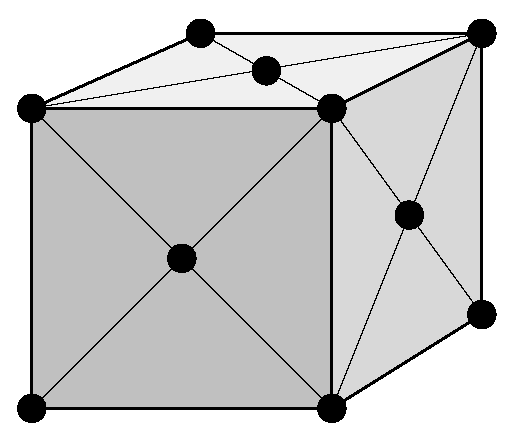
\includegraphics[width=3cm]{fcc.eps}
\end{center}
Create a visualization of an fcc lattice with a single species of atom
(such as occurs in metallic iron, for instance).
\end{enumerate}


%%% Exercise 3.5 %%%

\exercise \textbf{Visualization of the solar system}

\exskip The innermost six planets of our solar system revolve around the
Sun in roughly circular orbits that all lie approximately in the same
(ecliptic) plane.  Here are some basic parameters:
\begin{center}
\setlength{\tabcolsep}{8pt}
\begin{tabular}{l|ccc}
       & Radius of object & Radius of orbit  & Period of orbit \\
Object &       (km)       & (millions of km) &     (days)      \\
\hline
Mercury & 2440                  & 57.9                             & 88.0                   \\
Venus   & 6052                  & 108.2                            & 224.7                  \\
Earth   & 6371                  & 149.6                            & 365.3                  \\
Mars    & 3386                  & 227.9                            & 687.0                  \\
Jupiter & 69173                 & 778.5                            & 4331.6                 \\
Saturn  & 57316                 & 1433.4                           & 10759.2                \\
Sun     & 695500                & --                               & --

\end{tabular}
\end{center}

\smallskip\noindent
Using the facilities provided by the \verb|visual| package, create an
animation of the solar system that shows the following:
\begin{enumerate}\setlength{\itemsep}{0pt}
\item The Sun and planets as spheres in their appropriate positions and
  with sizes proportional to their actual sizes.  Because the radii of the
  planets are tiny compared to the distances between them, represent the
  planets by spheres with radii $c_1$ times larger than their correct
  proportionate values, so that you can see them clearly.  Find a good
  value for $c_1$ that makes the planets visible.  You'll also need to find
  a good radius for the Sun.  Choose any value that gives a clear
  visualization.  (It doesn't work to scale the radius of the Sun by the
  same factor you use for the planets, because it'll come out looking much
  too large.  So just use whatever works.)  For added realism, you may also
  want to make your spheres different colors.  For instance, Earth could be
  blue and the Sun could be yellow.
\item The motion of the planets as they move around the Sun (by making the
  spheres of the planets move).  In the interests of alleviating boredom,
  construct your program so that time in your animation runs a factor of
  $c_2$ faster than actual time.  Find a good value of $c_2$ that makes the
  motion of the orbits easily visible but not unreasonably fast.  Make use
  of the \verb|rate| function to make your animation run smoothly.
\end{enumerate}
Hint: You may find it useful to store the sphere variables representing the
planets in an array of the kind described on page~115.

\exercise \textbf{Deterministic chaos and the Feigenbaum plot}

\exskip One of the most famous examples of the phenomenon of chaos is the
\defn{logistic map}, defined by the equation
\begin{equation}
x' = rx(1-x).
\end{equation}
For a given value of the constant~$r$ you take a value of~$x$---say
$x=\half$---and you feed it into the right-hand side of this equation,
which gives you a value of~$x'$.  Then you take that value and feed it back
in on the right-hand side again, which gives you another value, and so
forth.  This is a \defn{iterative map}.  You keep doing the same
operation over and over on your value of~$x$, and one of three things
happens: {\renewcommand{\labelenumi}{\arabic{enumi}.\ }
\begin{enumerate}\setlength{\itemsep}{0pt}
\item The value settles down to a fixed number and stays there.  This is
  called a \defn{fixed point}.  For instance, $x=0$ is always a
  fixed point of the logistic map.  (You put $x=0$ on the right-hand side
  and you get $x'=0$ on the left.)
\item It doesn't settle down to a single value, but it settles down into a
  periodic pattern, rotating around a set of values, such as say four
  values, repeating them in sequence over and over.  This is called a
  \defn{limit cycle}.
\item It goes crazy.  It generates a seemingly random sequence of numbers
  that appear to have no rhyme or reason to them at all.  This is
  \defn{deterministic chaos}.  ``Chaos'' because it really does look
  chaotic, and ``deterministic'' because even though the values look
  random, they're not.  They're clearly entirely predictable, because they
  are given to you by one simple equation.  The behavior is
  \emph{determined}, although it may not look like it.
\end{enumerate}}
Write a program that calculates and displays the behavior of the logistic
map.  Here's what you need to do.  For a given value of~$r$, start with
$x=\half$, and iterate the logistic map equation a thousand times.  That
will give it a chance to settle down to a fixed point or limit cycle if
it's going to.  Then run for another thousand iterations and plot the
points $(r,x)$ on a graph where the horizontal axis is~$r$ and the vertical
axis is~$x$.  You can either use the \verb|plot| function with the options
\verb|"ko"| or \verb|"k."| to draw a graph with dots, one for each point,
of you can use the \verb|scatter| function to draw a scatter plot (which
always uses dots).  Repeat the whole calculation for values of $r$ from 1
to~4 in steps of~0.01, plotting the dots for all values of~$r$ on the same
figure and then finally using the function \verb|show| once to display the
complete figure.

Your program should generate a distinctive plot that looks like a tree bent
over onto its side.  This famous picture is called the
\defn{Feigenbaum plot}, after its discoverer Mitchell
Feigenbaum, or sometimes the \defn{figtree plot}, a play on the fact
that it looks like a tree and Feigenbaum means ``figtree'' in
German.

Give answers to the following questions:
\begin{enumerate}\setlength{\itemsep}{0pt}
\item For a given value of~$r$ what would a fixed point look like on the
  Feigenbaum plot?  How about a limit cycle?  And what would chaos look
  like?
\item Based on your plot, at what value of~$r$ does the system move from
  orderly behavior (fixed points or limit cycles) to chaotic behavior?
  This point is sometimes called the ``edge of chaos.''
\end{enumerate}

The logistic map is a very simple mathematical system, but deterministic
chaos is seen in many more complex physical systems also, including
especially fluid dynamics and the weather.  Because of its apparently
random nature, the behavior of chaotic systems is difficult to predict and
strongly affected by small perturbations in outside conditions.  You've
probably heard of the classic exemplar of chaos in weather systems, the
\defn{butterfly effect}, which was popularized by physicist Edward Lorenz
in 1972 when he gave a lecture to the American Association for the
Advancement of Science entitled, ``Does the flap of a butterfly's wings in
Brazil set off a tornado in Texas?''  (Although arguably the first person
to suggest the butterfly effect was not a physicist at all, but the science
fiction writer Ray Bradbury in his famous 1952 short story \textit{A Sound
  of Thunder}, in which a time traveler's careless destruction of a
butterfly during a tourist trip to the Jurassic era changes the course of
history.)

\medskip \textbf{Comment:} There is another approach for computing the
Feigenbaum plot, which is neater and faster, making use of Python's ability
to perform arithmetic with entire arrays.  You could create an
array~\Verb|r| with one element containing each distinct value of~$r$ you
want to investigate: \Verb|[1.0, 1.01, 1.02, ... ]|.  Then create another
array~\Verb|x| of the same size to hold the corresponding values of~$x$,
which should all be initially set to~$0.5$.  Then an iteration of the
logistic map can be performed for all values of~$r$ at once with a
statement of the form \Verb|x = r*x*(1-x)|.  Because of the speed with
which Python can perform calculations on arrays, this method should be
significantly faster than the more basic method above.


\exercise \textbf{The Mandelbrot set}

\exskip The Mandelbrot set, named after its discoverer, the French
mathematician Beno\^{\i}t Mandelbrot, is a \defn{fractal}, an infinitely
ramified mathematical object that contains structure within structure
within structure, as deep as we care to look.  The definition of the
Mandelbrot set is in terms of complex numbers as follows.

Consider the equation
\begin{displaymath}
z' = z^2 + c,
\end{displaymath}
where $z$ is a complex number and $c$ is a complex constant.  For any given
value of $c$ this equation turns an input number~$z$ into an output
number~$z'$.  The definition of the Mandelbrot set involves the repeated
iteration of this equation: we take an initial starting value of~$z$ and
feed it into the equation to get a new value~$z'$.  Then we take that value
and feed it in again to get another value, and so forth.  The Mandelbrot
set is the set of points in the complex plane that satisfies the following
definition:
\begin{quote}
\it For a given complex value of~$c$, start with $z=0$ and iterate
repeatedly.  If the magnitude~$|z|$ of the resulting value is ever greater
than~2, then the point in the complex plane at position~$c$ is \emph{not}
in the Mandelbrot set, otherwise it is in the set.
\end{quote}
In order to use this definition one would, in principle, have to iterate
infinitely many times to prove that a point is in the Mandelbrot set, since
a point is in the set only if the iteration never passes $|z|=2$ ever.  In
practice, however, one usually just performs some large number of
iterations, say 100, and if $|z|$ hasn't exceeded 2 by that point then we
call that good enough.

Write a program to make an image of the Mandelbrot set by performing the
iteration for all values of $c=x+\ii y$ on an $N\times N$ grid spanning the
region where $-2\le x\le 2$ and $-2\le y\le 2$.  Make a density plot in
which grid points inside the Mandelbrot set are colored black and those
outside are colored white.  The Mandelbrot set has a very distinctive shape
that looks something like a beetle with a long snout---you'll know it when
you see it.

Hint: You will probably find it useful to start off with quite a coarse
grid, i.e.,~with a small value of~$N$---perhaps $N=100$---so that your
program runs quickly while you are testing it.  Once you are sure it is
working correctly, increase the value of $N$ to produce a final
high-quality image of the shape of the set.

If you are feeling enthusiastic, here is another variant of the same
exercise that can produce amazing looking pictures.  Instead of coloring
points just black or white, color points according to the number of
iterations of the equation before $|z|$ becomes greater than~2 (or the
maximum number of iterations if $|z|$ never becomes greater than~2).  If
you use one of the more colorful color schemes Python provides for density
plots, such as the ``\verb|hot|'' or ``\verb|jet|'' schemes, you can make
some spectacular images this way.  Another interesting variant is to color
according to the logarithm of the number of iterations, which helps reveal
some of the finer structure outside the set.


%%% Exercise 3.6 %%%

\exercise \textbf{Least-squares fitting and the photoelectric effect}

\exskip It's a common situation in physics that an experiment produces data
that lies roughly on a straight line, like the dots in this figure:
\medskip\begin{center}
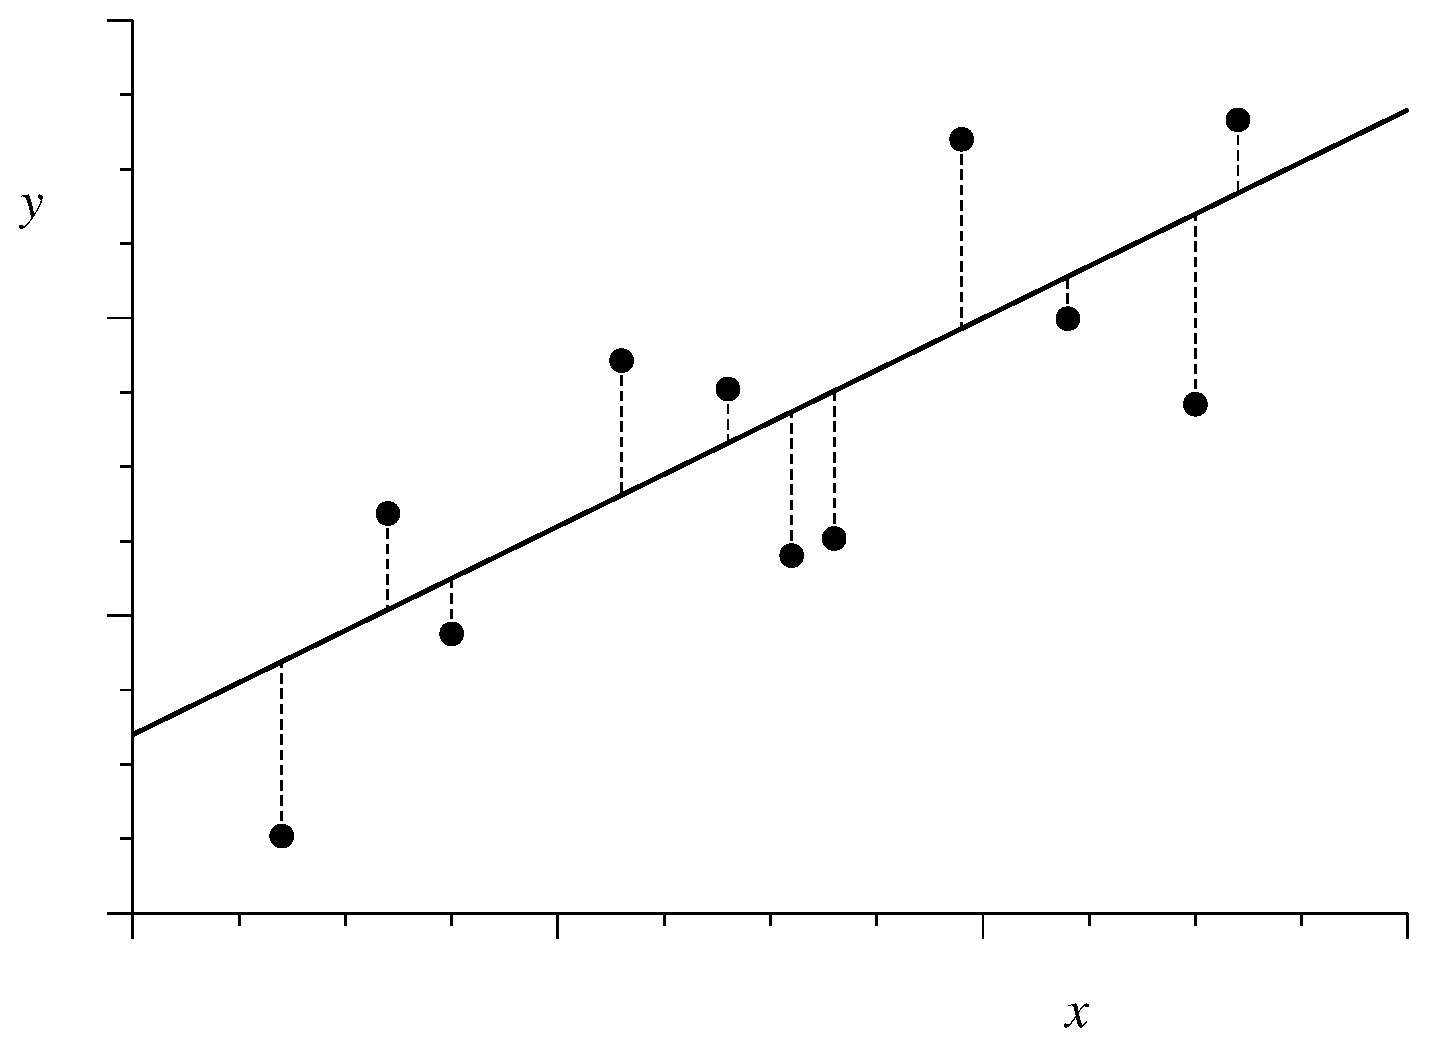
\includegraphics[width=10cm]{leastsq.eps}
\end{center}
The solid line here represents the underlying straight-line form, which we
usually don't know, and the points representing the measured data lie
roughly along the line but don't fall exactly on it, typically because of
measurement error.

The straight line can be represented in the familiar form $y=mx+c$ and a
frequent question is what the appropriate values of the slope~$m$ and
intercept~$c$ are that correspond to the measured data.  Since the data
don't fall perfectly on a straight line, there is no perfect answer to such
a question, but we can find the straight line that gives the best
compromise fit to the data.  The standard technique for doing this is the
\defn{method of least squares}.

Suppose we make some guess about the parameters~$m$ and $c$ for the
straight line.  We then calculate the vertical distances between the data
points and that line, as represented by the short vertical lines in the
figure, then we calculate the sum of the squares of those distances, which
we denote~$\chi^2$.  If we have $N$ data points with
coordinates~$(x_i,y_i)$, then $\chi^2$~is given by
\begin{displaymath}
\chi^2 = \sum_{i=1}^N (mx_i+c-y_i)^2.
\end{displaymath}
The least-squares fit of the straight line to the data is the straight line
that minimizes this total squared distance from data to line.  We find the
minimum by differentiating with respect to both $m$ and~$c$ and setting the
derivatives to zero, which gives
\begin{align*}
m \sum_{i=1}^N x_i^2 + c \sum_{i=1}^N x_i - \sum_{i=1}^N x_iy_i &= 0, \\
m \sum_{i=1}^N x_i + cN - \sum_{i=1}^N y_i &= 0.
\end{align*}
For convenience, let us define the following quantities:
\begin{displaymath}
E_x = {1\over N} \sum_{i=1}^N x_i,\qquad
E_y = {1\over N} \sum_{i=1}^N y_i,\qquad
E_{xx} = {1\over N} \sum_{i=1}^N x_i^2,\qquad
E_{xy} = {1\over N} \sum_{i=1}^N x_iy_i,
\end{displaymath}
in terms of which our equations can be written
\begin{align*}
mE_{xx} + cE_x &= E_{xy}\,, \\
mE_x + c &= E_y\,.
\end{align*}
Solving these equations simultaneously for $m$ and $c$ now gives
\begin{displaymath}
m = {E_{xy}-E_x E_y\over E_{xx} - E_x^2},\qquad
c = {E_{xx}E_y-E_x E_{xy}\over E_{xx} - E_x^2}.
\end{displaymath}
These are the equations for the least-squares fit of a straight line to $N$
data points.  They tell you the values of $m$ and~$c$ for the line that
best fits the given data.

\begin{enumerate}\setlength{\itemsep}{0pt}
\item In the on-line resources you will find a file called
  \verb|millikan.txt|.  The file contains two columns of numbers, giving
  the $x$ and $y$ coordinates of a set of data points.  Write a program to
  read these data points and make a graph with one dot or circle for each
  point.
\item Add code to your program, before the part that makes the graph, to
  calculate the quantities $E_x$, $E_y$, $E_{xx}$, and~$E_{xy}$ defined
  above, and from them calculate and print out the slope~$m$ and
  intercept~$c$ of the best-fit line.
\item Now write code that goes through each of the data points in turn and
  evaluates the quantity~$mx_i+c$ using the values of $m$ and $c$ that you
  calculated.  Store these values in a new array or list, and then graph
  this new array, as a solid line, on the same plot as the original data.
  You should end up with a plot of the data points plus a straight line
  that runs through them.
\item The data in the file \verb|millikan.txt| are taken from a historic
  experiment by Robert Millikan that measured the
  \defn{photoelectric effect}.  When light of an appropriate wavelength is
  shone on the surface of a metal, the photons in the light can strike
  conduction electrons in the metal and, sometimes, eject them from the
  surface into the free space above.  The energy of an ejected electron is
  equal to the energy of the photon that struck it minus a small
  amount~$\phi$ called the \defn{work function} of the surface,
  which represents the energy needed to remove an electron from the
  surface.  The energy of a photon is~$h\nu$, where $h$ is Planck's
  constant and $\nu$ is the frequency of the light, and we can measure the
  energy of an ejected electron by measuring the voltage~$V$ that is just
  sufficient to stop the electron moving.  Then the voltage, frequency, and
  work function are related by the equation
\begin{displaymath}
V = {h\over e}\nu - \phi,
\end{displaymath}
where $e$ is the charge on the electron.  This equation was first given by
Albert Einstein in 1905.

The data in the file \verb|millikan.txt| represent frequencies~$\nu$ in
hertz (first column) and voltages~$V$ in volts (second column) from
photoelectric measurements of this kind.  Using the equation above and the
program you wrote, and given that the charge on the electron is
$1.602\times10^{-19}\,$C, calculate from Millikan's experimental data a
value for Planck's constant.  Compare your value with the accepted value of
the constant, which you can find in books or on-line.  You should get a
result within a couple of percent of the accepted value.
\end{enumerate}
This calculation is essentially the same as the one that Millikan himself
used to determine of the value of Planck's constant, although, lacking a
computer, he fitted his straight line to the data by eye.  In part for this
work, Millikan was awarded the Nobel prize in physics in 1923.

\end{exercises}

\end{document}
